% Options for packages loaded elsewhere
\PassOptionsToPackage{unicode}{hyperref}
\PassOptionsToPackage{hyphens}{url}
%
\documentclass[
  ignorenonframetext,
  aspectratio=169]{beamer}
\usepackage{pgfpages}
\setbeamertemplate{caption}[numbered]
\setbeamertemplate{caption label separator}{: }
\setbeamercolor{caption name}{fg=normal text.fg}
\beamertemplatenavigationsymbolsempty
% Prevent slide breaks in the middle of a paragraph
\widowpenalties 1 10000
\raggedbottom
\setbeamertemplate{part page}{
  \centering
  \begin{beamercolorbox}[sep=16pt,center]{part title}
    \usebeamerfont{part title}\insertpart\par
  \end{beamercolorbox}
}
\setbeamertemplate{section page}{
  \centering
  \begin{beamercolorbox}[sep=12pt,center]{part title}
    \usebeamerfont{section title}\insertsection\par
  \end{beamercolorbox}
}
\setbeamertemplate{subsection page}{
  \centering
  \begin{beamercolorbox}[sep=8pt,center]{part title}
    \usebeamerfont{subsection title}\insertsubsection\par
  \end{beamercolorbox}
}
\AtBeginPart{
  \frame{\partpage}
}
\AtBeginSection{
  \ifbibliography
  \else
    \frame{\sectionpage}
  \fi
}
\AtBeginSubsection{
  \frame{\subsectionpage}
}
\usepackage{amsmath,amssymb}
\usepackage{lmodern}
\usepackage{iftex}
\ifPDFTeX
  \usepackage[T1]{fontenc}
  \usepackage[utf8]{inputenc}
  \usepackage{textcomp} % provide euro and other symbols
\else % if luatex or xetex
  \usepackage{unicode-math}
  \defaultfontfeatures{Scale=MatchLowercase}
  \defaultfontfeatures[\rmfamily]{Ligatures=TeX,Scale=1}
\fi
\usecolortheme{whale}
% Use upquote if available, for straight quotes in verbatim environments
\IfFileExists{upquote.sty}{\usepackage{upquote}}{}
\IfFileExists{microtype.sty}{% use microtype if available
  \usepackage[]{microtype}
  \UseMicrotypeSet[protrusion]{basicmath} % disable protrusion for tt fonts
}{}
\makeatletter
\@ifundefined{KOMAClassName}{% if non-KOMA class
  \IfFileExists{parskip.sty}{%
    \usepackage{parskip}
  }{% else
    \setlength{\parindent}{0pt}
    \setlength{\parskip}{6pt plus 2pt minus 1pt}}
}{% if KOMA class
  \KOMAoptions{parskip=half}}
\makeatother
\usepackage{xcolor}
\IfFileExists{xurl.sty}{\usepackage{xurl}}{} % add URL line breaks if available
\IfFileExists{bookmark.sty}{\usepackage{bookmark}}{\usepackage{hyperref}}
\hypersetup{
  pdftitle={CSHS Workshop: R for hydrologists - projects},
  pdfauthor={Kevin Shook; Paul Whitfield; Daniel Moore},
  hidelinks,
  pdfcreator={LaTeX via pandoc}}
\urlstyle{same} % disable monospaced font for URLs
\newif\ifbibliography
\usepackage{graphicx}
\makeatletter
\def\maxwidth{\ifdim\Gin@nat@width>\linewidth\linewidth\else\Gin@nat@width\fi}
\def\maxheight{\ifdim\Gin@nat@height>\textheight\textheight\else\Gin@nat@height\fi}
\makeatother
% Scale images if necessary, so that they will not overflow the page
% margins by default, and it is still possible to overwrite the defaults
% using explicit options in \includegraphics[width, height, ...]{}
\setkeys{Gin}{width=\maxwidth,height=\maxheight,keepaspectratio}
% Set default figure placement to htbp
\makeatletter
\def\fps@figure{htbp}
\makeatother
\setlength{\emergencystretch}{3em} % prevent overfull lines
\providecommand{\tightlist}{%
  \setlength{\itemsep}{0pt}\setlength{\parskip}{0pt}}
\setcounter{secnumdepth}{-\maxdimen} % remove section numbering
\titlegraphic{\centering 
\includegraphics[width=4cm]{figures/cshslogo_2019.png}}
\ifLuaTeX
  \usepackage{selnolig}  % disable illegal ligatures
\fi

\title{CSHS Workshop: R for hydrologists - projects}
\subtitle{CWRA 2022}
\author{Kevin Shook \and Paul Whitfield \and Daniel Moore}
\date{June 4, 2022}
\institute{Canadian Society for Hydrological Sciences (CSHS)}

\begin{document}
\frame{\titlepage}

\begin{frame}[fragile]{Why create a project?}
\protect\hypertarget{why-create-a-project}{}
\begin{itemize}
\tightlist
\item
  Makes your code more reproducible
\item
  Keeps code separate from other projects
\item
  Lets your code work with \texttt{git} and \textbf{GitHub}
\item
  Basis for creating packages
\end{itemize}
\end{frame}

\begin{frame}{How to create a project}
\protect\hypertarget{how-to-create-a-project}{}
\begin{itemize}
\tightlist
\item
  Command is \textbf{File \textbar{} New Project}
\item
  Several alternatives appear
\end{itemize}

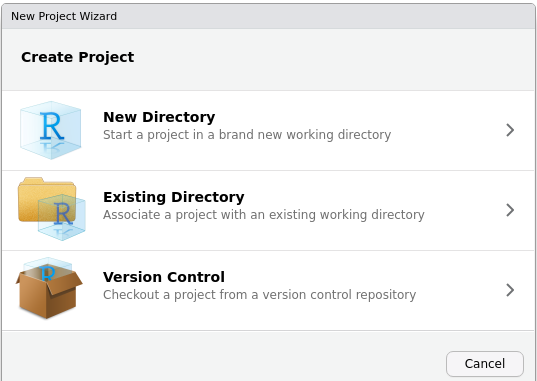
\includegraphics[width=0.5\textwidth,height=\textheight]{figures/new_project.png}
\end{frame}

\begin{frame}{Decisions, decisions\ldots.}
\protect\hypertarget{decisions-decisions.}{}
\begin{itemize}
\tightlist
\item
  New Directory

  \begin{itemize}
  \tightlist
  \item
    allows you to create any type of project, including packages
  \item
    can use \textbf{git} (always a good idea), \emph{but}
  \item
    \emph{won't} work with \textbf{GitHub}
  \end{itemize}
\item
  Existing Directory

  \begin{itemize}
  \tightlist
  \item
    only creates a simple project
  \item
    doesn't set up \textbf{git}, but you can add it later
  \item
    \emph{won't} work with \textbf{GitHub}
  \end{itemize}
\item
  Version Control

  \begin{itemize}
  \tightlist
  \item
    clones a project from a repository like \textbf{GitHub} or
    \textbf{GitLab}
  \item
    project has to be set up on the repository \emph{first}
  \end{itemize}
\end{itemize}
\end{frame}

\begin{frame}[fragile]{.Rproj file}
\protect\hypertarget{rproj-file}{}
\begin{itemize}
\tightlist
\item
  Every project contains a project file (\texttt{project\_name.Rproj})

  \begin{itemize}
  \tightlist
  \item
    a text file which contains the project settings
  \end{itemize}
\item
  Double-clicking on the file in your file manager will load
  \textbf{RStudio} with the project

  \begin{itemize}
  \tightlist
  \item
    default directory will be set to the project directory
  \end{itemize}
\item
  Can also load a project manually in \textbf{RStudio} using\\
  \textbf{File \textbar{} Open Project} or\\
  \textbf{File \textbar{} Recent Projects}
\item
  You can only have one project open at a time

  \begin{itemize}
  \tightlist
  \item
    opening a project will close your current project
  \end{itemize}
\end{itemize}
\end{frame}

\begin{frame}{git}
\protect\hypertarget{git}{}
\begin{itemize}
\tightlist
\item
  \textbf{git} is a program for version control
\item
  Created by Linus Torvalds (creator of Linux)
\item
  Allows you to manage versions of your documents
\item
  \textbf{RStudio} allows you to do most operations without typing
  commands

  \begin{itemize}
  \tightlist
  \item
    if you screw up, you \emph{will} have to type \textbf{git} commands
  \end{itemize}
\item
  Can sync with \textbf{GitHub}
\end{itemize}
\end{frame}

\begin{frame}{Working with git}
\protect\hypertarget{working-with-git}{}
\begin{itemize}
\tightlist
\item
  \textbf{git} is based on \emph{branches}

  \begin{itemize}
  \tightlist
  \item
    each branch is a separate set of files
  \end{itemize}
\item
  There is always a \textbf{main} (or \textbf{master}) branch

  \begin{itemize}
  \tightlist
  \item
    best version of the files
  \end{itemize}
\item
  When a branch is ready, it can be merged into the \textbf{main} branch
\item
<<<<<<< HEAD
  You can switch between branches at any time
\end{itemize}
\end{frame}

\begin{frame}{git branches}
\protect\hypertarget{git-branches}{}
\begin{itemize}
\tightlist
\item
=======
>>>>>>> 9cc47c4cecefde3535c7cc3b3b6101b167483ecd
  \emph{ALWAYS} create a new branch before working on a project

  \begin{itemize}
  \tightlist
  \item
<<<<<<< HEAD
    if you don't it will be a huge PITA
  \end{itemize}
\item
  Click on \textbf{New Branch} button in the \textbf{Git} tab
  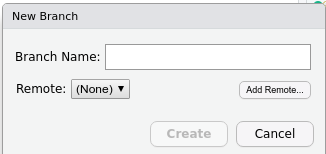
\includegraphics{figures/new_branch.png}
\end{itemize}
\end{frame}

\begin{frame}{Committing}
\protect\hypertarget{committing}{}
\begin{itemize}
\tightlist
\item
  When you have finished some work, you can commit your changes by
\item
  selecting the files to commit and
\item
  clicking on \textbf{Commit} in the \textbf{Git} tab
\item
  You will then see a window which lets you review your changes
\item
  You \textbf{must} type a Commit message describing your changes before
  clicking on the Commit button 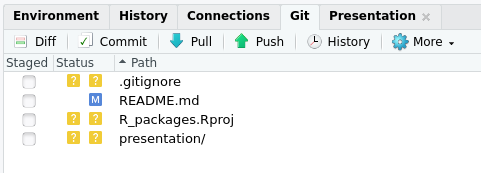
\includegraphics{figures/commit.png}
\end{itemize}
\end{frame}

\begin{frame}{Exercise}
\protect\hypertarget{exercise}{}
\begin{itemize}
\tightlist
\item
  Create a new project in a new directory
\item
  Check ``Create a git repository''
\item
  Don't check ``Use renv with this project''

  \begin{itemize}
  \tightlist
  \item
    \textbf{renv} is a package which keeps copies of all of the packages
    that you use with the project
  \end{itemize}
\item
  Quit \textbf{RStudio}
\item
  Copy the file ``f2c.R'' to the project directory
\item
  Copy the file ``Introduction\_to\_R\_Tutorial.Rmd'' to the project
  directory
\item
  Go to your file manager and double-click on the ``.Rproj'' file in the
  new directory

  \begin{itemize}
  \tightlist
  \item
    you should now see ``f2c.R'' in the Files tab
  \end{itemize}
\item
  Create a new branch in the Git tab

  \begin{itemize}
  \tightlist
  \item
    load ``f2c.R''
  \item
    make an edit to the file ``f2c.R''
  \item
    commit the change
  \end{itemize}
\item
  In \textbf{RStudio} click on \textbf{File \textbar{} Recent Projects}
  to re-load \emph{this} project
\end{itemize}
\end{frame}

\begin{frame}[fragile]{GitHub}
\protect\hypertarget{github}{}
\begin{itemize}
\tightlist
\item
  You can sync your project with an online repository at GitHub or
  GitLab
\item
  Have to set up the online repo \emph{first}

  \begin{itemize}
  \tightlist
  \item
    need an account
  \item
    have to have \texttt{ssh} set up on your computer
  \end{itemize}
\item
  When you create a project, you select Version Control
\end{itemize}

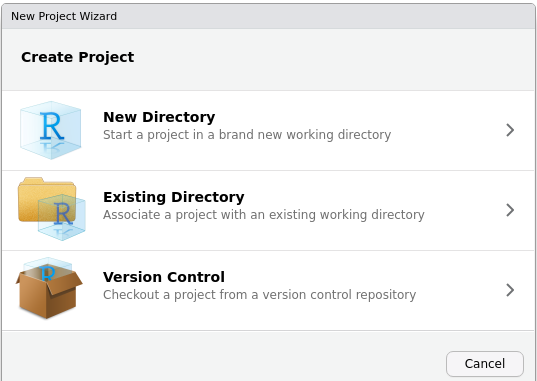
\includegraphics[width=0.4\textwidth,height=\textheight]{figures/new_project.png}
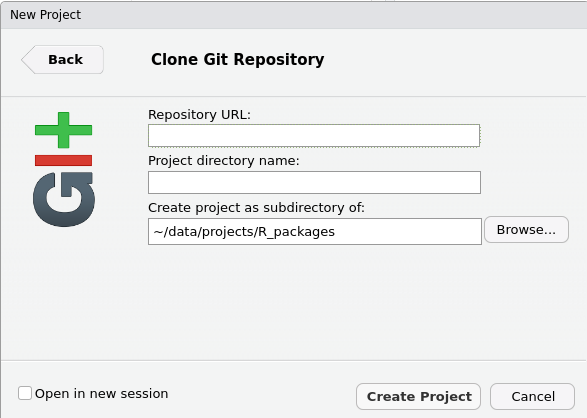
\includegraphics[width=0.4\textwidth,height=\textheight]{figures/git.png}
\end{frame}

\begin{frame}{\textbf{R} Packages}
\protect\hypertarget{r-packages}{}
\begin{itemize}
\tightlist
\item
  \textbf{R} packages are special types of projects
\item
  Only hold functions - do \emph{not} use them for Notebooks
\item
  Have
=======
    if you don't it will be a PITA
  \end{itemize}
>>>>>>> 9cc47c4cecefde3535c7cc3b3b6101b167483ecd
\end{itemize}
\end{frame}

\end{document}
